\chapter{Langevin Simulations}
\label{chap:langevinsimulations}

To illustrate the wealth of information and form prior distributions for the confined diffusion model, we can simulate the diffusion process of a control molecule diffusing in a confined electrostatic environment. 

The goal of this project was to model the diffusion process of confined diffusion using literature, and utilize pre-existing theory to for a statistical estimator of surface charge from diffusion dynamics.

\section{Simulation Equations}

The simulation scheme follows that described in \cite{millanNumericalSimulationsConfined2023}. A brownian particle diffuses between two walls such that $(x,y)$ are perpendicular to the walls, and $z$ is parallel. The electrostatic force that the particle feels is then only in the $z$ direction. The diffusivity of the particle will depend on the distance of the walls. The Langevin equation simulated, 
\begin{equation}
    m\ddot{\vec{x}}(t) = - \gamma(z) \dot{\vec{x}}(t) + \vec F(\vec{x}(t)) + \sqrt{2k_b T \gamma(z)} \vec{W}(t),
\end{equation}
is first separated into transverse and axial components, where $F$ is the electrostatic force, $\gamma$ is the friction. Here, we can re-write the diffusion coefficient using the Stokes-Einstein relation,
\begin{equation}
    D(z) = \frac{k_b T}{\gamma(z)}.
\end{equation}

Then, in over-damped regime, where $m \ddot{\vec{x}} \ll 0$, we can write the equations of motion as
\begin{equation}
    \begin{aligned}
        \frac{dx}{dt} &= \sqrt{2D_x(z)} W_x(t) \\
        \frac{dz}{dt} &= \sqrt{2D_z(z)} W_z(t) + \frac{F_z(z)}{\gamma(z)},
    \end{aligned}
\end{equation}
as described in Eqn. 7 of \cite{millanNumericalSimulationsConfined2023}. This is exceptionally valid for particles between $\SI{10}{\nm} - \SI{100}{\micro \meter}$ as this is exactly the over-damped regime for many particle materials, such as PMMA or coated polystyrene.

To simulate this equation, we use an Euler-Maruyama scheme. To illustrate this, we can rewrite the above equations in the Ito form, replacing lowercase variables with their capital, stochastic, equivalents:
\begin{equation}
    \begin{aligned}
        dX_t &= \sqrt{2D_x(z)} dW_x \\
        dZ_t &= \sqrt{2D_z(z)} dW_z + \frac{F_z(z)}{\gamma(z)} dt,
    \end{aligned}
\end{equation}

The simulated system of equations is then the pair of equations;
\begin{equation}
    \begin{aligned}
        x_{n+1} &= x_n + \sqrt{2D_x(z_n)} W_{x,n}\Delta t\\
        z_{n+1} &= z_n + \left[D'_z(z_n) - \beta D_z(z_n) V'(z_n) + \sqrt{2D_z(z_n)} W_{x,n}\right]\Delta t\\
    \end{aligned}
\end{equation}
where $V(z)$ is the electrostatic potential, $\beta = 1/k_b T$, and $\Delta t$ is the discretized time. 

\section{Surface Charge Estimator}

As described earlier, the relations for the effective potential are described if one knows the particle properties and surface charge. In terms of measurable electrostatic interactions can be fully described by the following  equation,

\begin{equation}
    U(z) = B\left[e^{-(H - z)/\lambda_D} - e^{-(H + z)/\lambda_D}\right],
\end{equation}
where the pre-factor is described by the map $f: (\zeta_p, \sigma_w, a, \lambda_D, T)$,
\begin{align}\label{eqn:electrostatic_forces}
    B &= C \cdot \tanh\left(\frac{e_0 \zeta_p}{4k_b T}\right) \cdot \tanh\left(\frac{e_0 \psi_w}{4k_b T}\right) \\
    C & = \frac{64 \pi \varepsilon_0 \varepsilon_r a k_b T}{e_0^2}\\
    \psi_w &= \frac{2k_b T}{e_0}\text{asinh}\left[\frac{\sigma_w e_0 \lambda_D}{2 \varepsilon_0 \varepsilon_r k_b T}\right]
\end{align}
where $\zeta_p$ is the zeta-potential of the particle, $\psi_w$ is the stern-layer potential for the surface walls, $a$ is the particle radius, $e_0$ is the elementary charge value, and $\lambda_D$ is the Debye-length. 

The surface charge of the walls can be estimated if one knows the electrostatic amplitude potential. Since the electrostatic force is a drift term, one can construct a maximum likelihood estimator as a standard result from the SDE. This estimator is derived in App. \ref{app:1}.

\begin{equation}
     \hat B = \frac{\sum_n \frac{\phi(z)}{2D_z}\left[\Delta z - D'(z)\Delta t\right]}{\sum_n \frac{\phi^2(z)\Delta t}{2D_z}} \quad, \mathbb{V}[\hat{B}] = \sum_{n=0}^\infty\frac{ \phi^2(z) \Delta t }{2D(z)}.
\end{equation}

If the amplitude of the electrostatic interactions is known, one can invert the amplitude using relations in Eqn. \ref{eqn:electrostatic_forces}. This inversion requires at least the zeta-potential of the particle, the size, and Debye-length. 

\section{Results}

We will simulate the priors of a Polystyrene bead diffusing with neutral charged walls, as well as those with varied levels of screening. In turn, we will be able to showcase the different cases of the known confined diffusion theory, as well as establishing prior curves for this work. In addition, the simulated curves will be compared to an effective theoretical model. For a given simulation, we can generate a realization of the dynamics following  the aforementioned SDEs. These realizations approach the Boltzmann limit as $t \gg \tau$. Some such realizations are shown in Fig. \ref{fig:brown_realization}

\begin{figure}[hb]
    \centering
    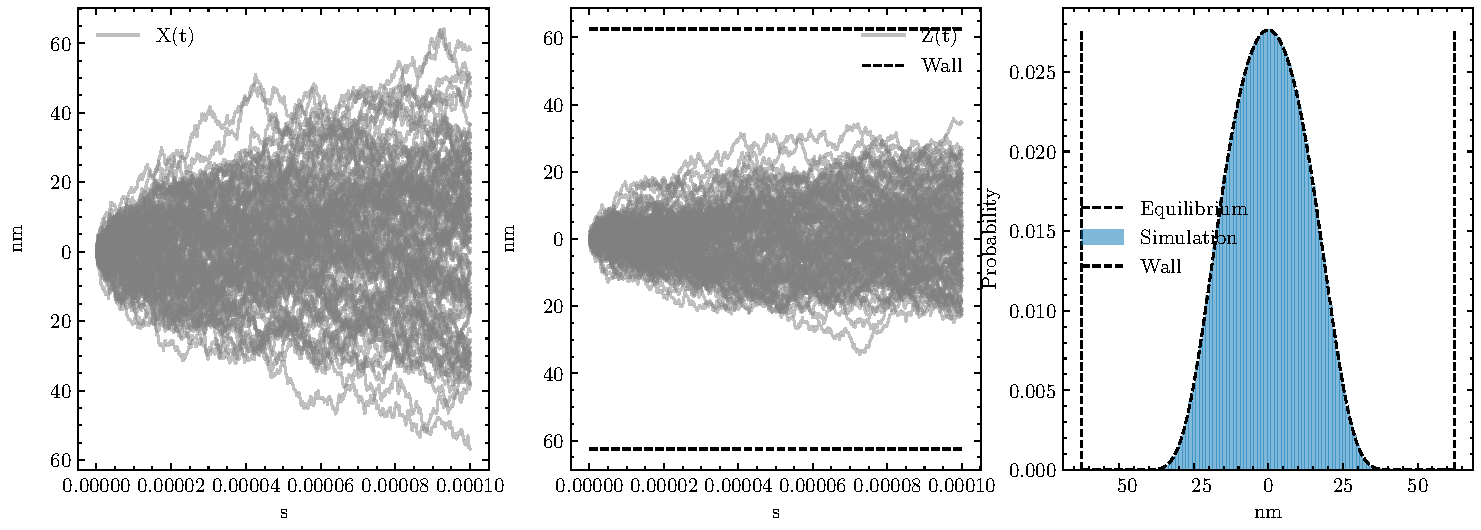
\includegraphics[width=\linewidth]{Figures/simulations/realization_and_boltzmann.pdf}
    \caption{Confined Brownian Particle realization of $z$ diffusion in electrostatic potential. $a = \SI{50}{\nm}, \zeta_p = \SI{-30}{\milli \volt}, \sigma_w = \SI{-2}{\milli \coulomb / \meter^2}, L = \SI{225}{\nm}, \lambda_D = \SI{10}{\nm}, T = \SI{300}{\kelvin}, \eta = \SI{1}{\milli \pascal \second}$. Left. Particle trajectory vs time for 100 realizations. Right. Histogram of steps vs. Boltzmann distribution.}
    \label{fig:brown_realization}
\end{figure}

\section{Mean-Squared Displacement in Confinement}

For a given experiment, one aims to measure something from knowing the trajectory of the particle. The simplest is an estimate of the size of the particle. One can do this using the transverse and axial trajectories obtained from the Langevin equation as a method to test the variance of the estimator given a known ground truth. In the case of an electrostatic potential, we can directly how measurements which do not account for screening effects change the measurement. 

\begin{figure}[h]
    \centering
    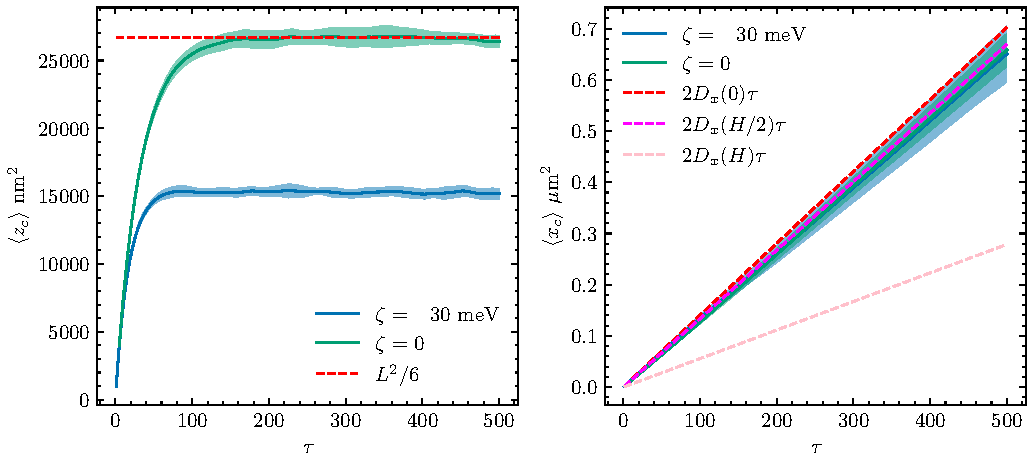
\includegraphics[width=\linewidth]{Python/Figures/xz_msd_comparison.pdf}
    \caption{Comparison between MSd curves of two highly different confined diffusors. Exposure time $\tau = \SI{200}{\micro \second}$, $\lambda_D = \SI{10}{\nm}$. }
    \label{fig:xz_msd_comparison}
\end{figure}

The notation of a higher confinement with respect to the zeta-potential is intrinsically linked to the electrostatic potential that the particle feels as it explores the well. This relationship between the effective confinement length can be solved by solving the Green's function for the FP-equation in the presence of an electrostatic potential. However, this happens to be non-analytical in the case of the Poisson-Boltzmann potential approximated in the Debye-Huckle theory. However, using the developed simulation class, this relationship can be directly measured. The same settings were used while fixing the zeta-potential of the particle, and varying the ionic concentration of the solution, which is inversely proportional to the Debye-length,
\begin{equation}
    \lambda_D \propto \frac{1}{\sqrt{C}},
\end{equation}
where $C$ is the ionic concentration of a dilute electrolyte compound [CITE]. To model this, the simulation settings are chosen as such $a = \SI{50}{\nm}, L = \SI{500}{\nm}, T = \SI{300}{\kelvin}, \Delta t_i = \SI{0.2}{\micro \second}, \tau = \SI{200}{\micro \second}, \eta = \SI{1}{\milli \pascal \second}$ and the Debye length is varied. The zeta potential of the particle and glass are chosen to resemble glass and a polystyrene bead, fixed at $\sigma_w = \SI{-2}{\milli \coulomb / \meter^2}, \zeta = \SI{-30}{\milli \volt}$. The relationship between the effective confinement length and the ionic concentration is shown in Fig. \ref{fig:conf_debyelen}

\begin{figure}
    \centering
    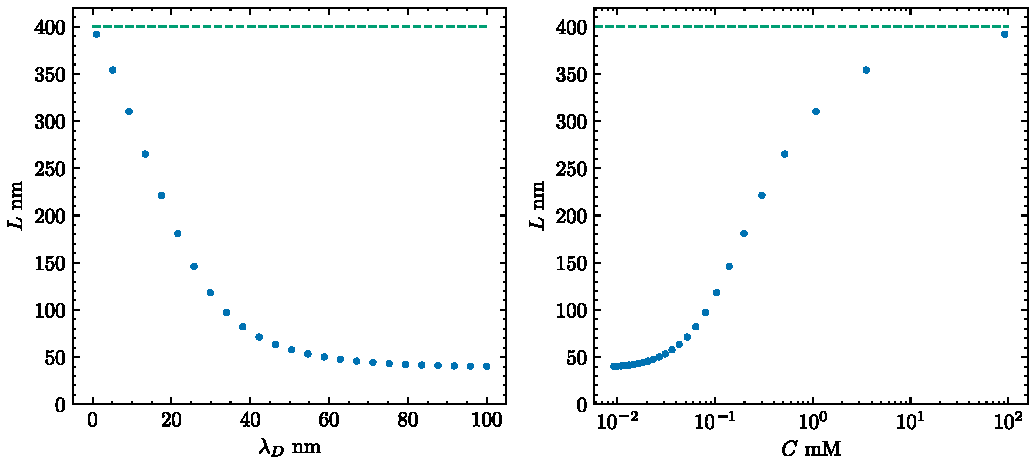
\includegraphics[width=\linewidth]{Python/Figures/conf_debyelength.pdf}
    \caption{Effective Confinement length plotted against the solution's Debye length. $a = \SI{50}{\nm}, L = \SI{500}{\nm}, T = \SI{300}{\kelvin}, \Delta t_i = \SI{0.2}{\micro \second}, \tau = \SI{200}{\micro \second}, \eta = \SI{1}{\milli \pascal \second}$ and the Debye length is varied. The zeta potential of the particle and glass are chosen to resemble glass and a polystyrene bead, fixed at $\sigma_w = \SI{-2}{\milli \coulomb / \meter^2}, \zeta = \SI{-30}{\milli \volt}$. }
    \label{fig:conf_debyelen}
\end{figure}

\begin{figure}
    \centering
    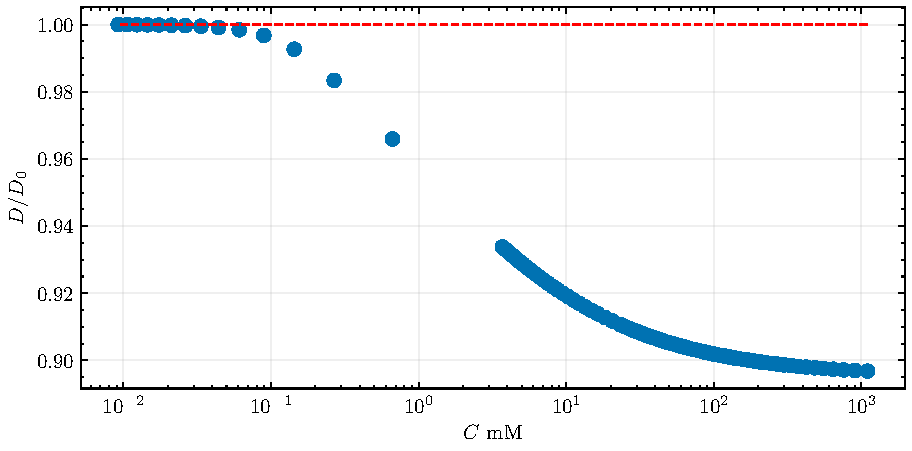
\includegraphics[width=\linewidth]{Python/Figures/diff_debye.pdf}
    \caption{Effective diffusion plotted against the solution's Debye length. $a = \SI{50}{\nm}, L = \SI{500}{\nm}, T = \SI{300}{\kelvin}, \Delta t_i = \SI{0.2}{\micro \second}, \tau = \SI{200}{\micro \second}, \eta = \SI{1}{\milli \pascal \second}$ and the Debye length is varied. The zeta potential of the particle and glass are chosen to resemble glass and a polystyrene bead, fixed at $\sigma_w = \SI{-2}{\milli \coulomb / \meter^2}, \zeta = \SI{-30}{\milli \volt}$. }
    \label{fig:diff_debyelen}
\end{figure}

The relationship between the effective confinement length, as well as the relationship between relative diffusion and concentration of ions begs the question of if this can be used as a particle filter to distinguish classes of particles. Here we investigate that question regarding the amount of confinement length compared to the zeta-potential of a particle at various Debye-lengths. This relationship is described in Fig. \ref{fig:conf_zeta_debye}.
\begin{figure}
    \centering
    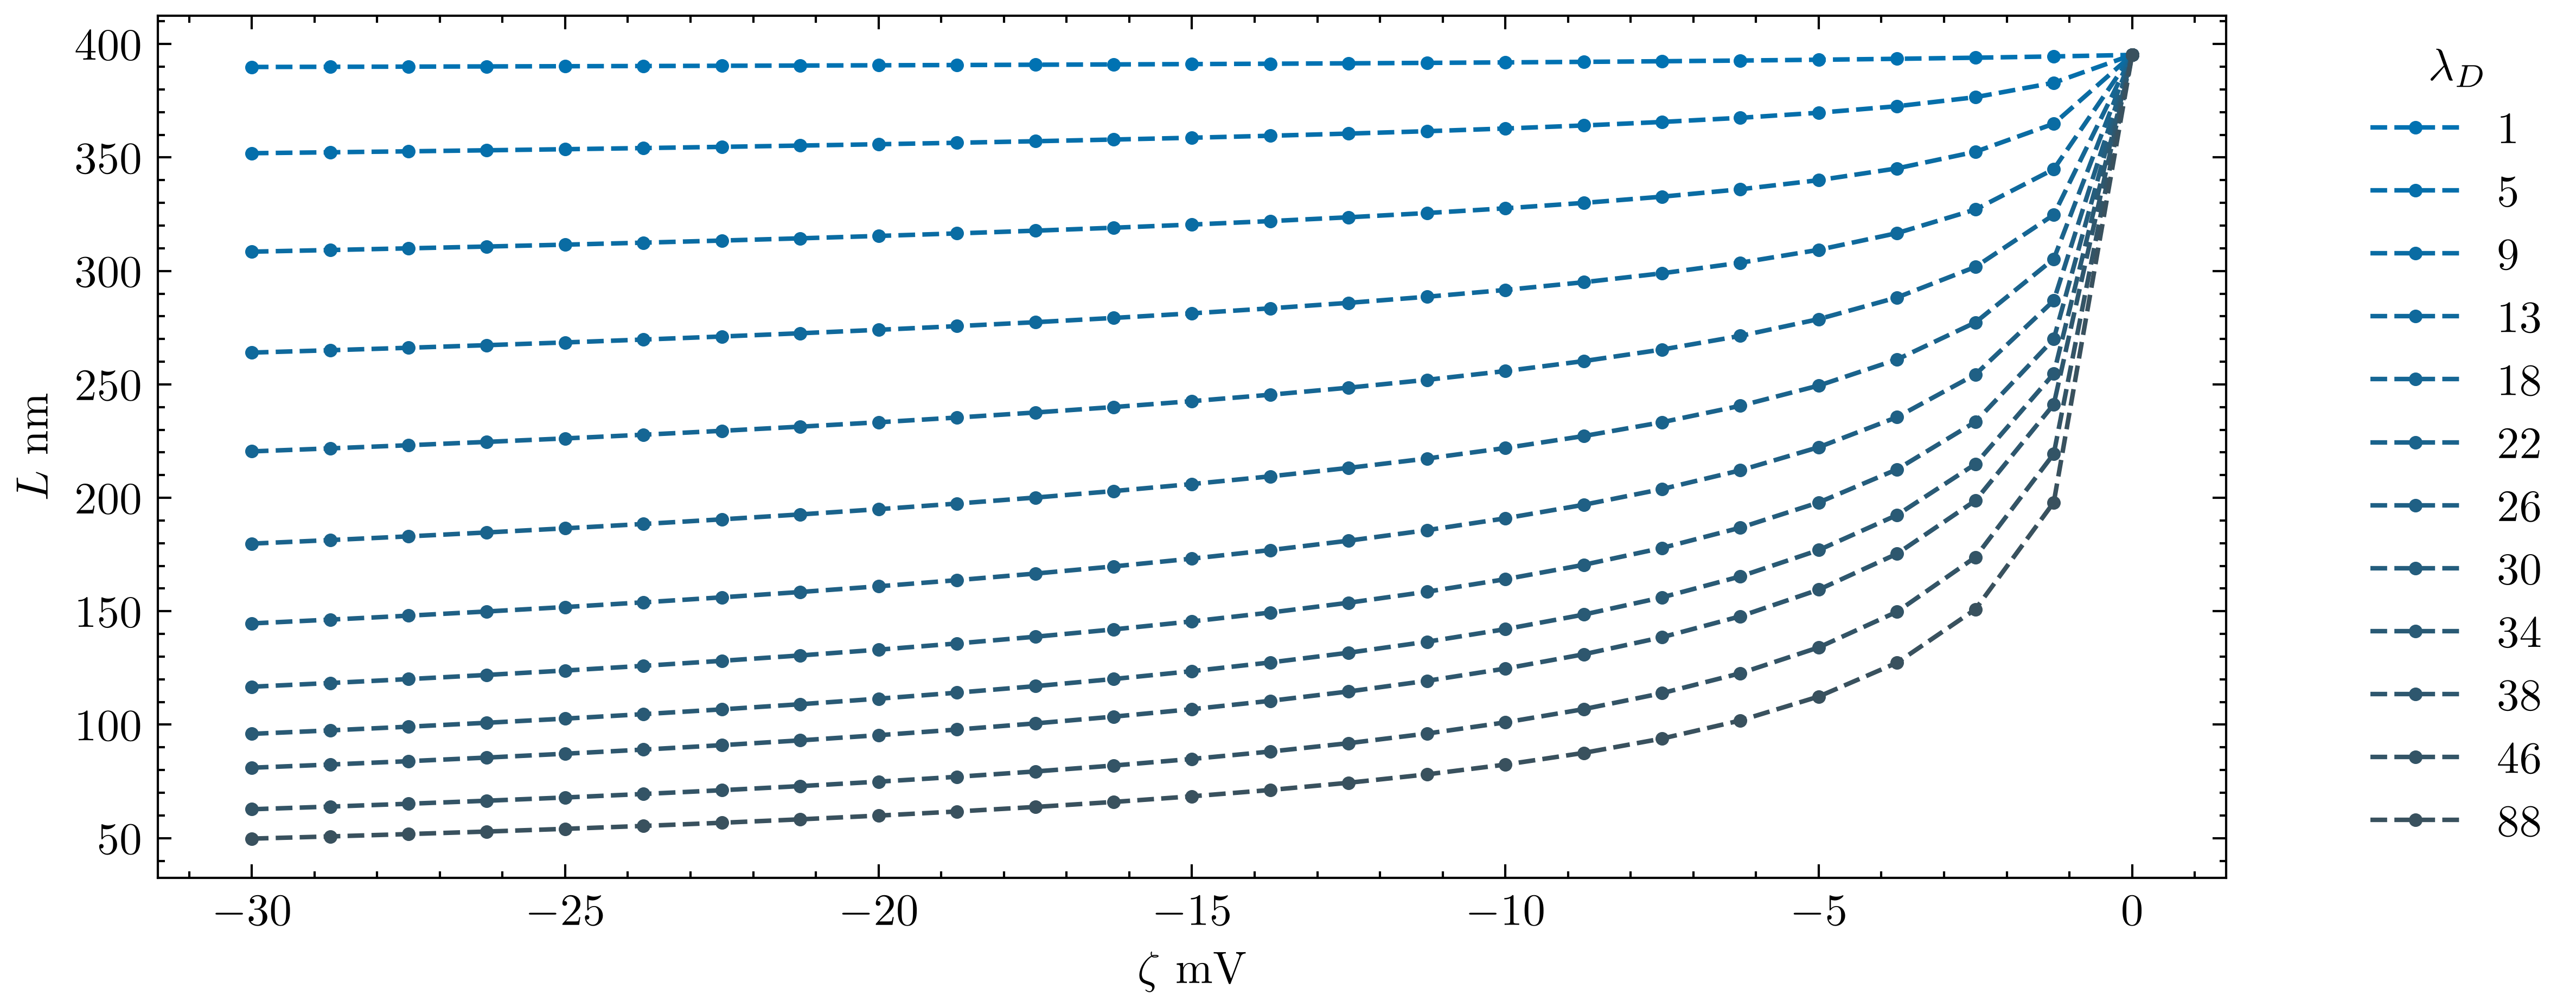
\includegraphics[width=\linewidth]{Python/Figures/conf_zeta_debye.png}
    \caption{Effective confinement plotted against the particle's zeta-potential. $a = \SI{50}{\nm}, L = \SI{500}{\nm}, T = \SI{300}{\kelvin}, \Delta t_i = \SI{0.2}{\micro \second}, \tau = \SI{200}{\micro \second}, \eta = \SI{1}{\milli \pascal \second}$ and the Debye length is varied. The surface charge of the wall are chosen to resemble glass, fixed at $\sigma_w = \SI{-2}{\milli \coulomb / \meter^2}$.}
    \label{fig:conf_zeta_debye}
\end{figure}

\section{Surface Charge estimation}

The particle's exploration demonstrated a clear dependence on a drift due to the electrostatics. This drift is a useful estimator of the particle-wall charge relationship. Using the aforementioned amplitude maximum-likelihood estimator, drift estimator can be extracted into meaningful, physical information. The Langevin simulation was ran for $\SI{20}{\ms}$ with time-step of $\SI{0.2}{\micro\second}$. The distribution of the MLE is shown in Fig \ref{fig:B_estimation}.

\begin{figure}[hb]
    \centering
    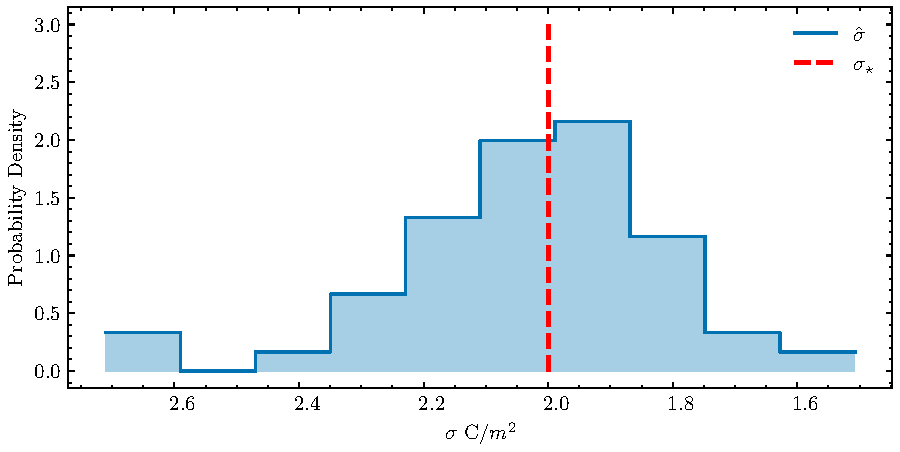
\includegraphics[width=0.75\linewidth]{Python/Figures/B_estimation_hist.pdf}
    \caption{Distribution of $\hat{B}$ Re-parameterized for the surface charge. $\hat{\sigma} = 1/(A\cdot C)^2 \hat{B}$ where $A,C$ are properly defined in \ref{eqn:electrostatic_forces}. In this histogram there are 50 simulations with seeds set to $S_{\text{eed}} = i* 10 + 1$ for $i \in \{0, 49\}$ using the \textit{numpy} seed parameter. $a = \SI{50}{\nm}, L = \SI{500}{\nm}, T = \SI{300}{\kelvin}, \Delta t_i = \SI{0.2}{\micro \second}, \tau = \SI{200}{\micro \second}, \eta = \SI{1}{\milli \pascal \second}, \lambda_D = \SI{10}{\nm}$ The surface charge is fixed at $\sigma_w = \SI{-2}{\milli \coulomb / \meter^2}$.}
    \label{fig:B_estimation}
\end{figure}

\section{Conclusion}

In conclusion, we have shown that confined simulations can be readily simulated with physical parameters as per literature. The simulations have shown that there are regions of instability in the Debye-surface charge regime where the confined diffusivity of the particles is maximally observed. For the case of polystyrene beads, this appears to be around $\lambda_D \approx \SI{80}{\nm}$. 

With regards of surface charge estimation, we have introduced a new MLE for the amplitude based on maximum likelihood estimation. The distribution has a mean centered around the ground truth with a standard deviation of $1/4 \cdot \sigma_\star$. 

\chapter{iSCAT z-estimation Simulations}
\label{chap:ZEstimation}

This section presents a computational method for determining the axial ($z$-axis) position of a nanoparticle from iSCAT imaging data. The proposed approach is based on principles of light-scattering in the Rayleigh approximation, which govern the inference pattern as the nanoparticle moves along the optical axis. 

In order to evaluate the accuracy and performance of the proposed method, Mie-theory simulations are used for for determining the an ideal nanoparticle's $z$-axis position. The precision and limitations are discussed in the context of recovering three-dimensional particle trajectories.

The raw images are acquired from a CMOS camera according the optical schematic illustrated in Figures \ref{fig:schematic} and \ref{fig:re_schematic}. Each image consists of a two-dimensional interference recorded at a specific focal position $z_\mathrm{focus}$, defined as the distance between the objective's focal distance and the objects in the field of view.

\section{Method Overview}

The method described in this section is based on computational image processing on images acquired using a CMOS camera. The camera has an array of $2048 \times 2048$ pixels. To acquire images at higher frame rates, only a portion of the CMOS array is used. This is set during the experimental details. Typical sizes used are $600 \times 450$ at $\SI{400}{\fps}$ however, other fields of view can be used for specific experimental purposes. The highest frame-rate possible with this camera is $\SI{1000}{\fps}$ at a FOV of $200 \times 250$.

The object sample is imaged through an oil-immersion objective lens. The optical system provides a magnification of $60 \times$, with a tube lens of magnification $2\times$. The remaining is an digital zoom with a final resolution of $\SI{55}{\nm}$ per pixel. The final magnification is then the ratio of the CMOS array length divided by the pixel size.

The image-processing workflow used to determine three-dimensional trajectory is shown in \ref{fig:method_outline}. The diagram summarized the sequence of image processing steps to extract each coordinate position.

\begin{figure}[h!]
    \centering
    \begin{minipage}{0.6\textwidth}
        \centering
        \begin{enumerate}
            \item Raw image captured on camera.
            \item Background subtraction to convert to iSCAT image.
            \item iSCAT $(x,y)$ Tracking
            \item Radial Integral to obtain scattering data.
            \item Nuisance parameter estimation to ensure physical stability.
            \item Particle axial position Linking with 2D chain-link algorithm.
            \item Axial position Extraction
            \item Three-dimensional trajectory is recovered.
        \end{enumerate}
    \end{minipage}
    \caption{Background subtraction outline. }
    \label{fig:method_outline}
\end{figure}


\section{Raw image background subtraction}

To obtain high-contrast interference signal from raw camera data, a post-processing background subtraction routine is introduced. This background subtraction measured a temporally averaged background using a window-filter and Fourier filtering. An example of this process is shown in Fig.\ref{fig:raw2iscat}.

\begin{figure}[h]
    \centering
    \begin{subfigure}[b]{0.8\textwidth}
        \centering
        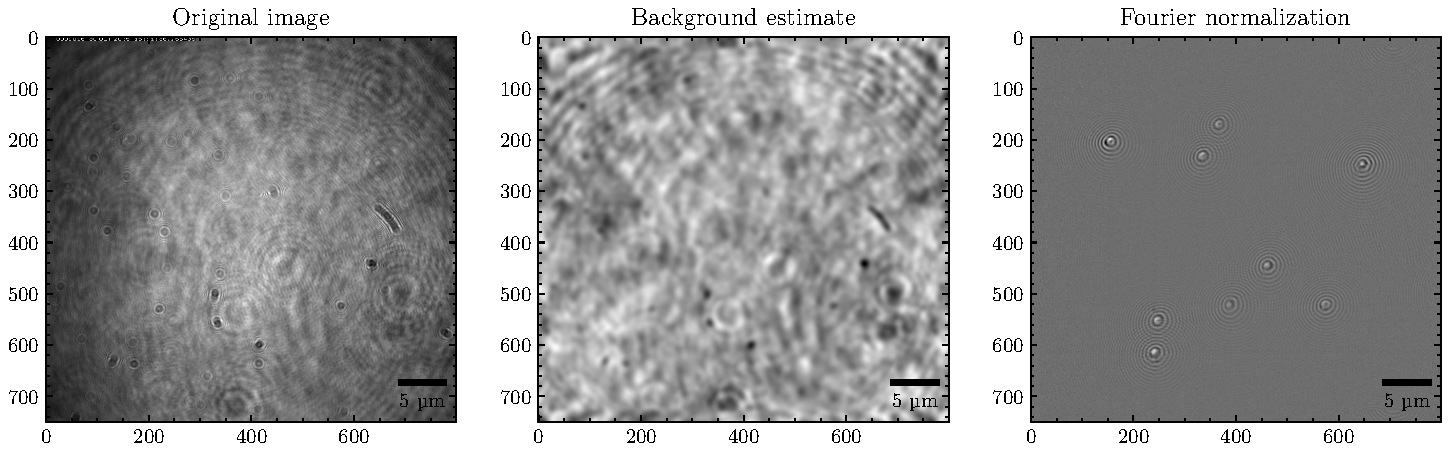
\includegraphics[width=\textwidth]{Python/Figures/NormalizationPipeline.pdf}
    \end{subfigure}
    
    \vspace{1em} % Adjust the vertical space between figures
    % Second (bottom) subfigure
    \begin{subfigure}[b]{0.5\textwidth}
        \centering
        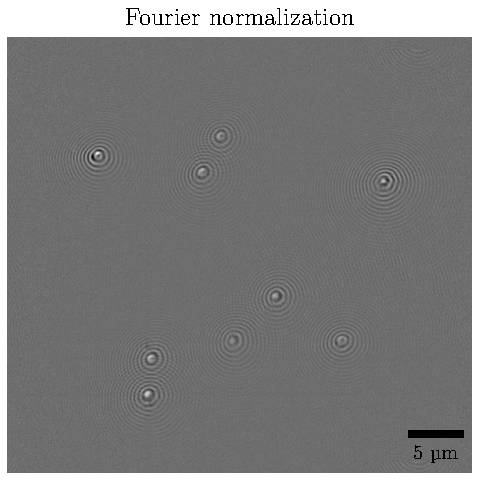
\includegraphics[width=\textwidth]{Python/Figures/NormalizationPipelineThird.pdf}
    \end{subfigure}

    \caption{Raw image captured on camera to background subtracted iSCAT image. Single particles are tracked and extracted for further analysis.}
    
    \label{fig:raw2iscat}
\end{figure}

The full algorithm is presented in Alg. \ref{alg:raw2iscat}. The overview of the algorithm is to subtract the background noise in order to minimize Poisson, and electronic noise. 

To reduce the contribution of the static background, the mean background is subtracted from each frame. Since the background illumination originates from the gaussian illumination beam, which has a constant mean intensity over the acquisition period, this stationary background removes the background offset while preserving dynamic iSCAT signal. This just requires a good estimation of the background in order not to remove any iSCAT signal. The remaining shot noise, which follows Poisson statistics is reduced by temporal averaging during background estimation. 

In order to suppress electronic noise from data-transfer, a row-wise averaging scheme is applied. Row-wise means are taken and normalized with respect to their row as the data-transfer from CMOS to computer is by horizontal lines. Thus, to ensure all lines are equally weighted, they are normalized with respect to their entire row. This is implemented as per prior iSCAT normalization methods by the Sandoghar laboratory \red{Vahid's github should be here.}

The set of images, which consist of matrices of pixel-values of shape $F \times H \times W$, or $F$ number of frames, $W$ pixels wide, $H$ pixels tall. 

Before processing begins, the parameters of the Fourier-band-pass filter are determined from the image dimensions. The filter consists of an annular, donut mask of inner radius equal to 1\% if the larger image dimension and outer radius equal to  25\% of the larger image dimension, corresponding to $r_i = \max(H,W)/100, r_o = \max(H,W)/4$. 

To minimize edge artifacts, a binary mask is applied to each frame. Pixels within 20 pixels of the boundary are assigned a value of 0 using a mask filter. On the interior pixels, the mask is set to $1$, while on the pixels less than 20 pixels away from the edge are set to 0. This mask is used during normalization to prevent edge effects from biasing the inner statistics.

For each frame in the stack, the image is first normalized using a row-wise normalization function. The function, titled \textsc{AmpNorm} in Alg. \ref{alg:raw2iscat}, first obtains the masked-image. The global normalized mean is stored. For each row, the mean is taken and the row of the global-mean is adjusted by the row-wise mean. The final image is the global mean divided by the row-mean for each row. 

Once normalized, the background of the image is calculated by taking the forward and backward $\Delta L$ frames spaced by a spacer of $\Delta f$ frames and taking the $\textsc{AmpNorm}$ of these frames. 

The iSCAT image then consists of a background subtraction between the normalized image and the background. Finally, once background subtracted, the image is Fourier-filtered using the pre-allocated band-pass filter. This process is demonstrated in Fig. \ref{fig:raw2iscat}

\section{iSCAT $(x, y)$ Tracking}

To determine the transverse positions of any particles detected in the iSCAT method, the radial variance transform algorithm is used \cite{kashkanovaPrecisionSingleparticleLocalization2021}. The original algorithm is briefly outlined below for completeness. The full code is written by the Sandoghdar group and can be found in Ref \cite{kashkanovaPrecisionSingleparticleLocalization2021}. A demonstration of this method is presented in the Fig. \ref{fig:transLoc}.

\begin{figure}[h]
    \centering
    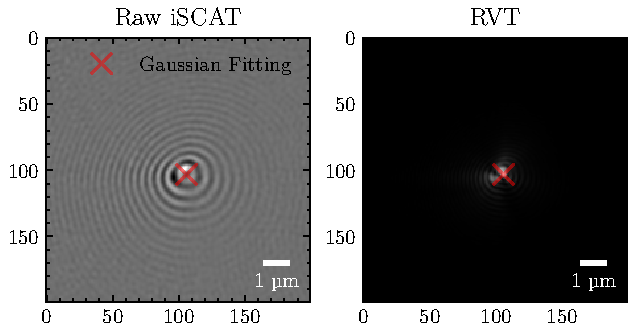
\includegraphics[width=\textwidth]{Python/Figures/Raw2RVT.pdf}
    \caption{Raw image to RVT. Gaussian fitting of the RVT is shown on both plots.}
    \label{fig:transLoc}
\end{figure}

The transverse localization algorithm, referenced as \textsc{TransverseLocalization} in \ref{alg:2d_track} consists of transformations onto the iSCAT image from the previous section. 

The input image stack is first loaded and assumed to consist of radially symmetric interference fringes. The image is first transformed using the Radial Variance Transform \cite{kashkanovaPrecisionSingleparticleLocalization2021}. This function converts a radial-fringe pattern into a point-like delta function when a radial symmetry is acted upon it. 

Before proceeding, a frame-independent parameter for threshold SNR amplitude, number of pixels, and ROI cropping parameters are inputted. for a particle to be detected, the SNR of the RVT should be roughly 90\% of the max iSCAT amplitude. An estimate of particle number is assumed, which acts as a prior for top $n$ detections. Lastly, ROI for sub-pixel estimation is chosen. 

For each frame, the iSCAT image is dilated. Particle positions that are considered maxima if the dilated image is equal to the RVT and the RVT is above the threshold for detection. 

Once candidates are chosen, a NL-LS gaussian fitting to the RVT is performed to acquire higher-accuracy localization. To improve this to sub-pixel, a crop is done around each RVT gaussian fitted point and a radial-symmetry algorithm is performed as per \cite{parthasarathyRapidAccurateParticle2012}.

\begin{figure}
    \centering
    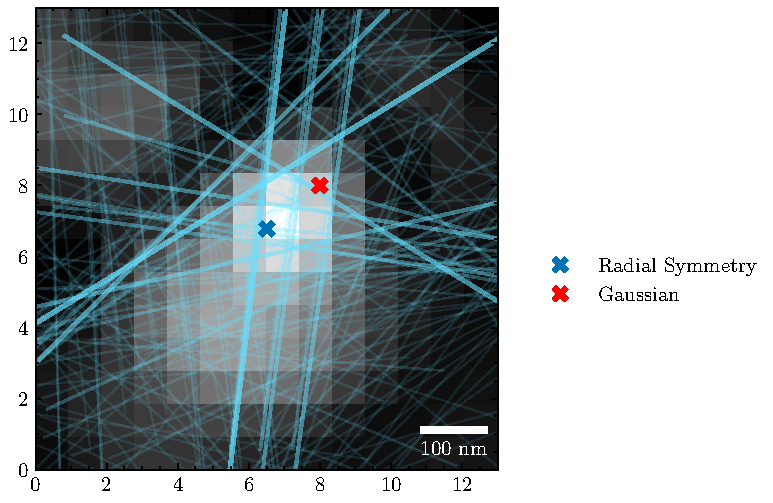
\includegraphics[width=0.8\textwidth]{Python/Figures/RadialSymExample.pdf}
    \caption{Demonstration of the Radial Symmetry method applied onto RVT of iSCAT data. Implemented from \cite{parthasarathyRapidAccurateParticle2012}. Figure adapted from \cite{parthasarathyRapidAccurateParticle2012}.  }
    \label{fig:RadialSym}
\end{figure}

To ensure accurate linking, an implementation of the \textsc{Munkres} algorithm is used \red{REF}. Briefly, a cost-matrix of distances is constructed and minimized in time to ensure that optimal displacements are chosen. This algorithm has limitations in cases where particles overlap. Ideally, experimental measure are taken to minimize this occurring. One such measure is to lower the concentration of particle in the recorded images. 



\section{Angular Integral}

Image data will have background misalignment due to iSCAT hardware setup. To optimize for fitting speed and misalignment property, radial scattering profile are assumed as in the Rayleigh regime model is symmetric. The radial integration method is described in Alg \ref{alg:rad_int}.

The discrete angular integral consists of summing angular terms on a radial grid. Mathematically, the output array obtained is described by the relation
\begin{equation}
    g_t(\rho) \tilde{-} \frac{1}{\Delta \theta}\int_{\theta_0}^{\theta_0 + \Delta \theta} I_t(\rho, \theta) d\theta,
\end{equation}
where $\theta_0$ is a constant, $\Delta \theta$ is the width of integration, $I_t(\rho, \theta)$ is the iSCAT image. 

First, the cartesian image is Re-parameterized into polar coordinates using a change of basis transformation on the index grid of the image. Then, for each ring of indices, the image coordinates are summed up on this ring. The final array is an angular average that is indexed at radius $r$ for some upper radial bound. This process is illustrated in Fig. \ref{fig:AngularInt}.

\begin{figure}[h!]
    \centering
    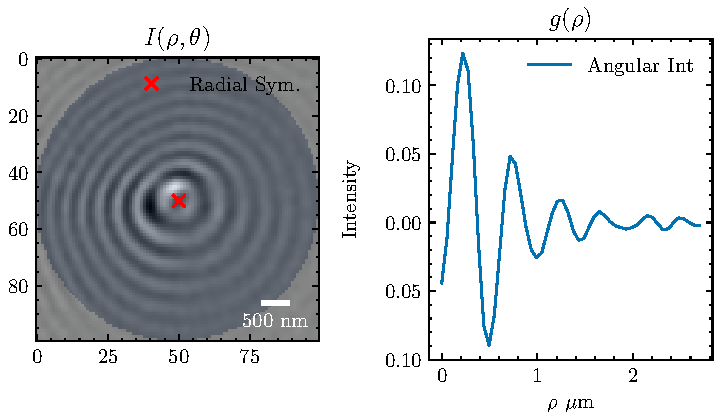
\includegraphics[width=\textwidth]{Python/Figures/AngularInt.pdf}
    \caption{Angular Integral demonstration.}
    \label{fig:AngularInt}
\end{figure}

\section{Nuisance parameter Estimation}

In order to speed up computation and produce a more statistically relevant result, the method aims to fix the model parameters which should theoretically stay constant. These, for example, are the particle mass signal and optical aberration coefficients. These parameters, known as nuisance parameters, should be fixed before fitting to the more sensitive parameter of interest, the relative $z$ position. 

To obtain accurate estimation of the $z$ position relative to nearby frames, nuisance estimation is done to focus on $z$ fitting. To do this, L-BFGS-B Fitting is performed. alongside amplitude fitting. The theory of nuisance parameter estimation is described in \cite{wasserman2010statistics}.

The nuisance parameter method works on the premise of a model function. The iPSF model described in \ref{chap:iscatprinciples} is used as a weight function to compare to the data. First, bounds are placed for physical values of each parameter.

Here, it is important to note that the amplitude of the signal is proportional to the mass. The spatial decay of the aberration is modeled as a decaying exponential.

For each candidate decay parameter, the weighted correlation function is calculated. Let $g$ be the radial profile, and $G$ the theoretical iPSF model. The inner product of these two arrays, weighted in some integral of radiuses, is defined by $\langle G, g \rangle_w$. The correlation function is then written as
\begin{equation}
    \rho(z, \gamma) = \frac{\langle G, g \rangle_w}{\sqrt{\langle G, G \rangle _w + \langle g, g \rangle_w + \varepsilon}},
\end{equation} 
where $\varepsilon$ is a small number to prevent division by 0. 

The best-fit amplitude function here is analytical, given by the expression
\begin{equation}
    \hat{E_0} = \frac{\langle G, g \rangle_w}{\langle G, G \rangle_w}.
\end{equation}

The loss-function, $\mathcal{L}$, given the correlation, is given by the subtraction of $\rho^2$,
\begin{equation}
    \mathcal{L} = 1-\rho^2(z, \gamma).
\end{equation}

Once a fitted $\gamma_0, \hat{E_0}$ are chosen, the optimal $z$ for each frame is given by a non-linear bounded least squares which are acquired using the L-BFGS-B method with a Huber Loss ($\delta = 1/2$). 

When computed for each frame in the stack, one has $F$ optimally chosen $\gamma_0, E_0$. To obtain the optimal parameter, a fit to distributions, inferred by \cite{dewitPreciseCharacterizationNanometerscale2023}, is used. These fits include a Gamma distribution for $E_0$ and a LogNorm distribution for $\gamma$. Together, these form nuisance estimation for $E_0, \gamma_0$.

\section{2D Chain-link}

Given an estimation of the nuisance parameters, a grid-search of the optimal $z$ is simple. The physically best $z$ position is a mean-squared error loss minima of the model subtracted with the data. However, due to the periodic nature of the data, there are up to 3 candidates for the optimal $z$ position based on $\lambda/4$ having a high degree of similarity. Thus, to resolve this, a z-linking method was implemented to find the most likely trace based on diffusion probabilities.

To link consequent positions in space, a dynamic programming algorithm is used. The algorithm is known as the Viterbi method and is described in Alg. \ref{alg:best_chain_2d}.

First, all minima for every frame must be collected. These are the candidate positions that trajectories are constructed from. The losses of these positions are also stored to ensure no spurious candidates are chosen. 

For each position, the forward pass compares all chains moving in time. The loss is accumulated by a weighted Euclidean transition cost,
\begin{equation}
    d_i(i,j) = \sqrt{w_x^2(x_{t-1}^(i) - x_{t}^(j))^2 + w_y^2(y_{t-1}^(i) - y_{t}^(j))^2},
\end{equation}
where $x$ denote $z$ motion, and $y$ denotes the loss difference. This matrix compares all weighted transitions. The optimal transition $\pi_t(j)$ is then chosen to minimize this transition, and any prior transitions. 

For each following forward pass, the cost is accumulated with a memory of 2 frames. The memory is chosen to ensure that an incorrect transition in a given frame is not penalized later on. 

Thus linking method is thus a search algorithm for the shortest math based on the weighted Euclidean method. A short toy-model is shown in Fig. \ref{fig:toyViterbi} to visualize the procedure.

\begin{figure}[H]
    \centering
    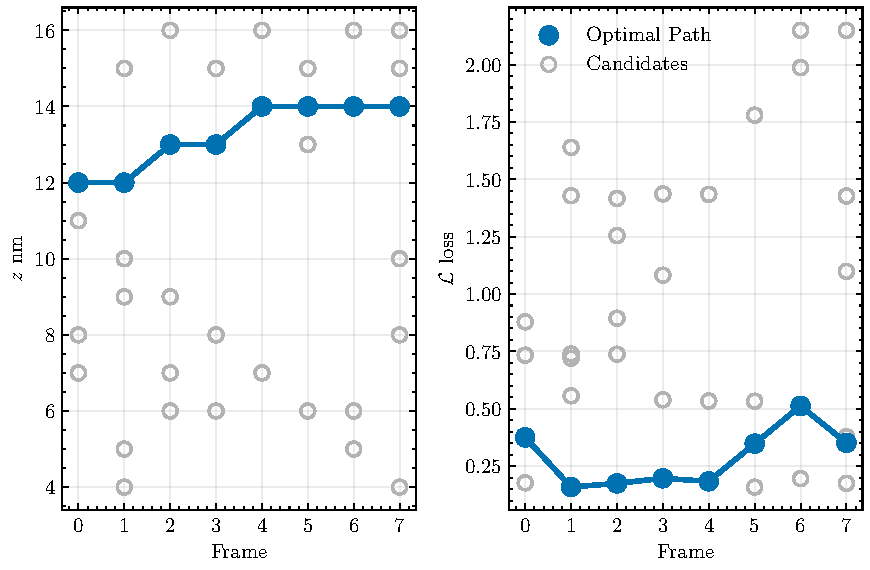
\includegraphics[width=0.8\textwidth]{Python/Figures/viterbi_toy.pdf}
    \caption{Viterbi Search algorithm toy example. Optimal path is chosen based on $z$ similarity and lowest loss.}
    \label{fig:toyViterbi}
\end{figure}

% \begin{algorithm}[H]
% \caption{Dynamic Programming for Best 2D Chain of Points}
% \label{alg:best_chain_2d}
% \begin{algorithmic}[1]
% \Require 
%     $\text{min\_idx} = \{ \text{min\_idx}[t] \}_{t=0}^{F-1}$, list of candidate positions per frame\\
%     $\text{min\_vals} = \{ \text{min\_vals}[t] \}_{t=0}^{F-1}$, list of candidate values per frame\\
%     $w = (w_x, w_y)$, weighting for distance computation (default $(1,1)$)\\
%     $\text{max\_step}$, optional maximum allowed step distance
% \Ensure
%     $\text{idx\_chain}, \text{x\_chain}, \text{y\_chain}$, the indices, positions, and values of the optimal path

% \State Initialize $F \gets |\text{min\_idx}|$
% \State Initialize $cost[i] \gets 0$ for all $i$ in frame $0$
% \State Initialize $prev \gets []$ \Comment{to store predecessor indices}

% \For{$t = 1$ to $F-1$}
%     \State $A_x \gets \text{min\_idx}[t-1]$, $B_x \gets \text{min\_idx}[t]$
%     \State $A_y \gets \text{min\_vals}[t-1]$, $B_y \gets \text{min\_vals}[t]$
%     \State Compute pairwise differences:
%         \[
%         \Delta_x[i,j] = |A_x[i] - B_x[j]|, \quad 
%         \Delta_y[i,j] = |A_y[i] - B_y[j]|
%         \]
%     \State Compute weighted Euclidean distances:
%         \[
%         D[i,j] = \sqrt{ (w_x \Delta_x[i,j])^2 + (w_y \Delta_y[i,j])^2 }
%         \]
%     \If{max\_step is not None}
%         \State Set $D[i,j] \gets \infty$ if $D[i,j] > \text{max\_step}$
%         \If{no finite $D[i,j]$ exists}
%             \State \Return empty path
%         \EndIf
%     \EndIf

%     \State Compute cumulative path cost matrix:
%         \[
%         M[i,j] = cost[i] + D[i,j]
%         \]
%     \State For each node $j$ in frame $t$, find predecessor $p[j]$ minimizing $M[:,j]$:
%         \[
%         p[j] = \arg\min_i M[i,j], \quad
%         new\_cost[j] = M[p[j], j]
%         \]
%     \State Update $cost \gets new\_cost$
%     \State Append $p$ to $prev$
% \EndFor

% \State Initialize $j \gets \arg\min_i cost[i]$  \Comment{index of minimal total cost in last frame}
% \State Initialize $\text{idx\_chain} \gets [0]^{F}$, set $\text{idx\_chain}[F-1] \gets j$
% \For{$t = F-2$ down to $0$}
%     \State $\text{idx\_chain}[t] \gets prev[t][\text{idx\_chain}[t+1]]$
% \EndFor

% \State Compute chains:
% \[
% \text{x\_chain}[t] = \text{min\_idx}[t][\text{idx\_chain}[t]], \quad
% \text{y\_chain}[t] = \text{min\_vals}[t][\text{idx\_chain}[t]]
% \]

% \State \Return $\text{idx\_chain}, \text{x\_chain}, \text{y\_chain}$
% \end{algorithmic}
% \end{algorithm}

\section{Simulated iPSF localization}

To validate the proposed method, one performs simulated axial-estimation. Simulated iSCAT point spread functions were generated using the \textsc{PiSCAT} library for $\lambda=\SI{405}{\nm}$. The iPSF was generated for the focal range $z_{f} \in [-1000, 0]$. The assumed particle is spherical with radius $a = \SI{50}{\nm}$. The iPSF is shown in Fig. \ref{fig:ipsf_sim}

\begin{figure}
    \centering
    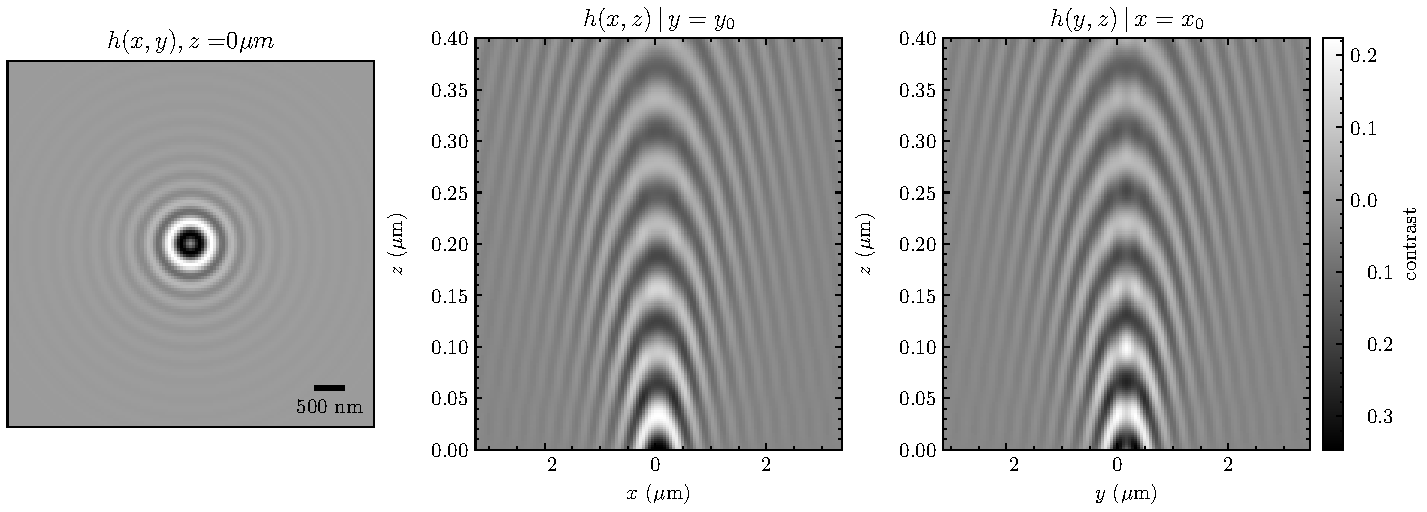
\includegraphics[width=\linewidth]{Python/Figures/sim_ipsf.pdf}
    \caption{Simulated iPSF. Left. Projection of in-focus plane. Middle. $x,z$ projection. Right. $y,z$ projection. Focal scan is over $\SI{400}{\nm}$. pixel size is $\SI{55}{\nm}/\text{pixel}$. $\lambda = \SI{405}{\nm}$. Assumed particle radius $a = \SI{50}{\nm}$.}
    \label{fig:ipsf_sim}
\end{figure}

As mentioned, the localization pipeline utilizes a weighting scheme to account for objective aberration and misalignments to non-modeled regions of the data, such as the central fringe. This is accounted for by using a binary weighting array, $\mathbf{w}$. In the case of these idealized simulations, we will show the effect of changing the weighting scheme as we proceed. This demonstrates a loss of absolute precision, however, maintains the relative precision, which is that of interest in measurements of axial trajectory. 

\section{3-parameter Estimation}

As a reminder, the model for the iPSF is a multivariate function $\text{iPSF}:(z, E_0, \gamma) \rightarrow \R^2$. It has been shown that the statistical model of $\text{iPSF}$ takes;
\begin{equation}
    \begin{aligned}
        \hat{E_0} &\sim \text{Gamma}(\mu_{E_0}, \sigma_{E_0}) \\
        \hat{\gamma} &\sim \text{logNorm}(\mu_{\gamma}, \sigma_{\gamma}) \\
    \end{aligned}
\end{equation}

The so-called 3-parameter estimation is a sampling of nuisance parameters in the model. The nuisance parameters here are $\hat{E_0}, \hat \gamma$, where $\hat{E_0}$ is an amplitude factor, and $\gamma$ is an exponential decay factor used to account for spatial decay in signal. The amplitude factor can be analytically solved for using a grid-search sweep along $z$. The $\gamma$ factor is fitted to using the L-BFGS-B minimization algorithm. This nuisance parameter fit is shown in the histograms of these two parameters shown in Fig. \ref{fig:nuisance_fit}.

\begin{figure}
    \centering
    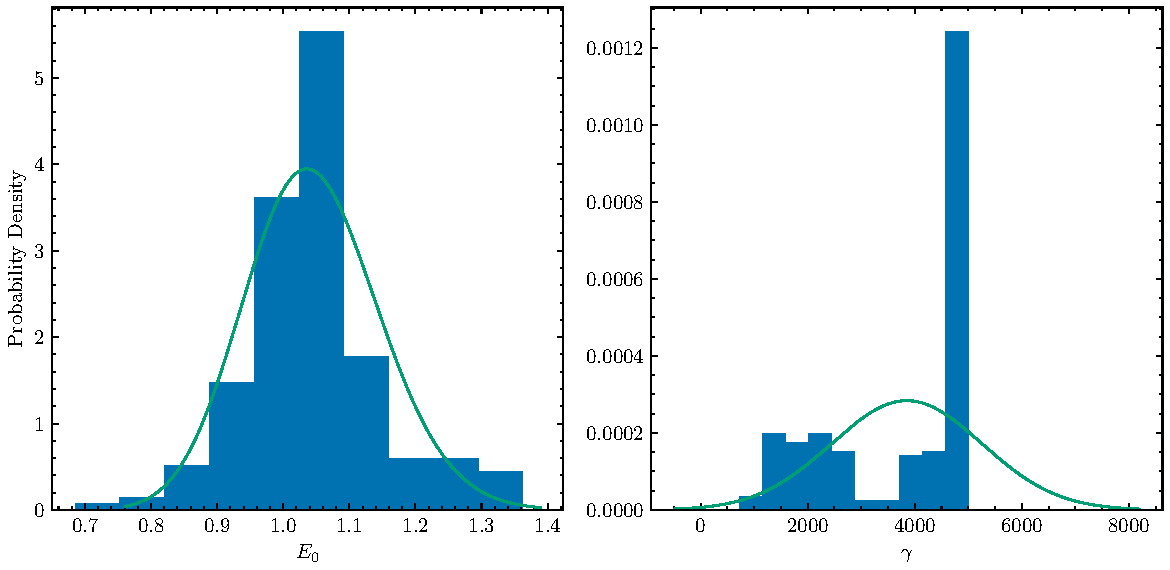
\includegraphics[width=\linewidth]{Python/Figures/nuisance_param.pdf}
    \caption{Nuisance Parameter estimation for iPSF fits. Left. Amplitude factor. right. exponential decay factor. The exponential decay is not of utmost importance as it often is very small. it is kept for stability purposes.}
    \label{fig:nuisance_fit}
\end{figure}

\subsection{Grid-Search Estimation}

Once the nuisance parameters are chosen, a grid-search with a dynamic linking is performed. Each frame is assumed to have a maximal diffusion time. This is in place to optimize for noise and have coherent, physical traces without outliers. The grid search takes the difference between the data and a scan over the model with the nuisance parameters in place. The best loss is chosen. In the case of linking, the minimal loss over the path is chosen. The full algorithm is discussed elsewhere. the residuals of this using no fitting are shown in Fig. \ref{fig:fit_residuals}.

\begin{figure}
    \centering
    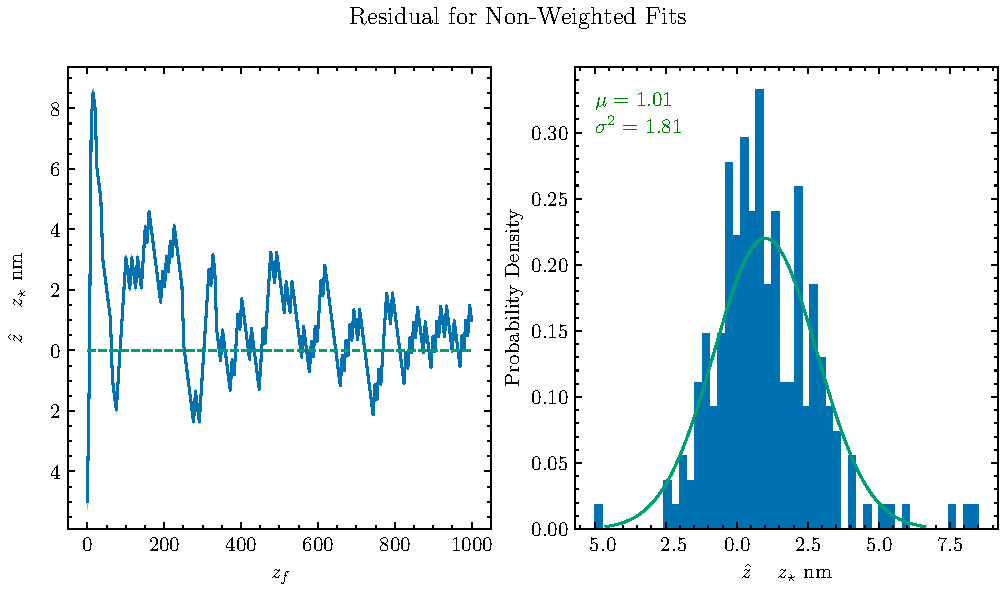
\includegraphics[width=\linewidth]{Python/Figures/simulation_fit_residual.pdf}
    \caption{Fit residuals using no weighting scheme. reporting an absolute bias of 1 nm with variance of 2 nanometers.}
    \label{fig:fit_residuals}
\end{figure}

\section{Conclusions}

In conclusion, the pseudocode for the method was outlined explicitly. The methodology was tested on simulation data with a high degree of accuracy. The method shows an accuracy of $\pm \SI{1}{\nm}$ with a forward bias of $\SI{1}{\nm}$.



